\documentclass{standalone}
\usepackage{pgfplots}
\pgfplotsset{compat=1.11}
\begin{document}
% Place the TikZ picture in a figure environment.
%\begin{figure}[htb]
% h: here, t: top, b: bottom, p: page of float
%% https://tex.stackexchange.com/questions/39017/how-to-influence-the-position-of-float-environments-like-figure-and-table-in-lat
%% ! indicates that some restrictions should be ignored (discussed later)
%% h indicates that the float is allowed to be placed inline
%% t indicates that the float is allowed to go into a top area
%% b indicates that the float is allowed to go into a bottom area
%% p indicates the the float is allowed to go on a float page or column area

    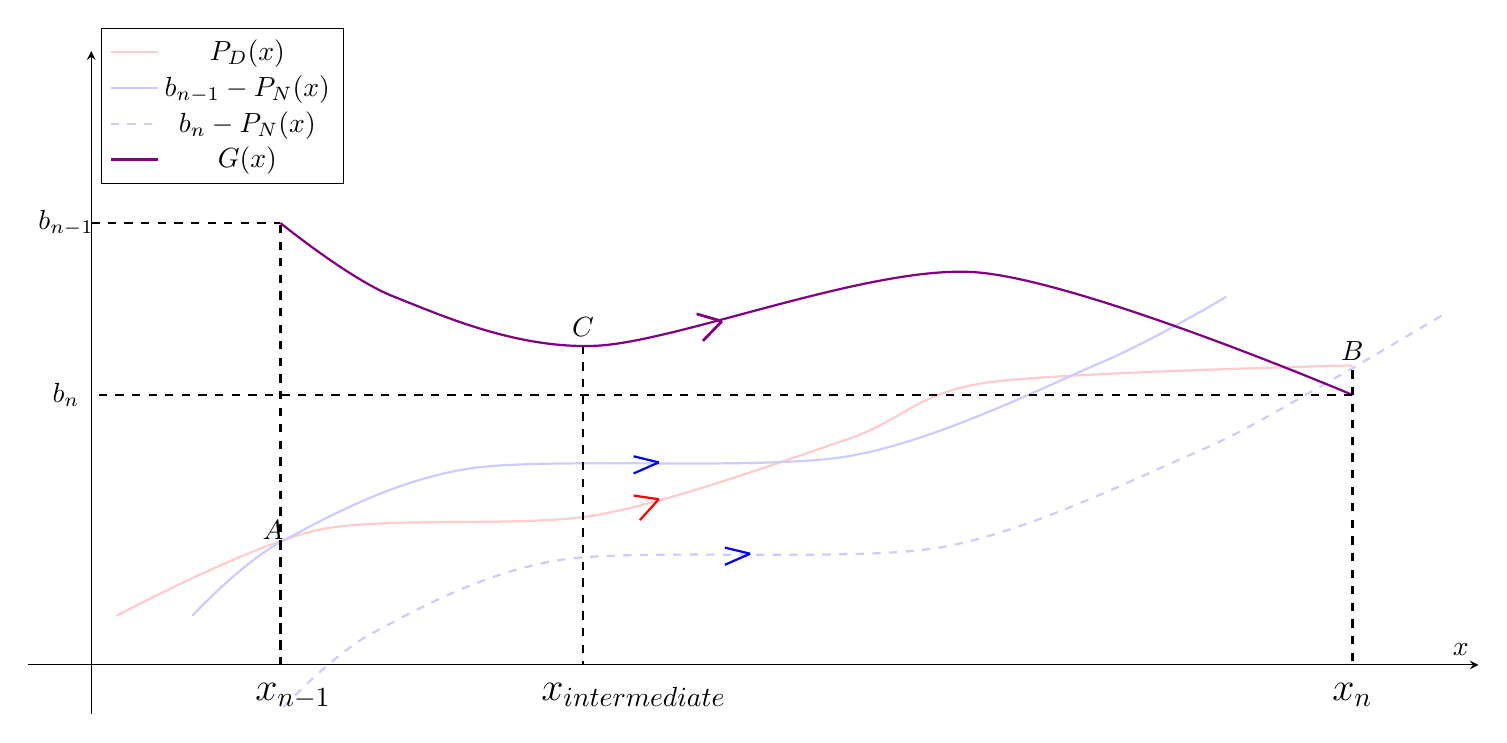
\begin{tikzpicture}
        \begin{axis} [
            height=10cm, width=20cm,
            xmin=-0.5, xmax=11, ymin=-0.2, ymax=2.5,
            xlabel={$x$},
                        % xtick={-2,-1.5,...,2}, ytick={-2,-1.5,...,2},
            xticklabel style={font=\tiny, xshift=0.5ex},
            yticklabel style={font=\tiny, yshift=0.5ex},
            axis line style={->},
            axis x line=middle,
            axis y line=middle,
            ticks=none,
            %grid=both,
           % legend pos=north west,
           legend style={at={(0.05,0.8)},anchor=south west}
        ]
         \draw [red!20,thick] plot [smooth,samples=200, tension=0.5] coordinates {(0.2,0.2) (1.8,0.55) (4, 0.61) (6, 0.92) (7.1,1.15) (10,1.22)};

        \addlegendimage{line width=0.3mm,color=red!20}
        \addlegendentry{$P_D(x)$}
   
        \draw [blue!20,thick] plot [smooth,samples=200, tension=0.5] coordinates { (0.8,0.2) (1.5,0.5) (3,0.8) (6,0.85) (8, 1.23) (9, 1.5) };

        \addlegendimage{line width=0.3mm,color=blue!20}
        \addlegendentry{$b_{n-1} - P_N(x)$}
        
        \draw [dashed,blue!20,thick][xshift=33pt,yshift=-33pt] plot [smooth,samples=200, tension=0.5] coordinates { (0.8,0.2) (1.5,0.5) (3,0.8) (6,0.85) (8, 1.23) (9,1.5) (10, 1.8)};
        
        \addlegendimage{line width=0.3mm,color=blue!20,dashed}
        \addlegendentry{$b_{n} - P_N(x)$}

        \draw [violet,thick] plot [smooth,samples=200, tension=0.5] coordinates {  (1.5,1.8) (2.4,1.5) (4,1.3) (7, 1.6) (10,1.1)};
    
        \addlegendimage{line width=0.3mm,color=violet}
        \addlegendentry{$G(x)$}
  
        \draw [-,thick,black, dashed] (10,1.1) -- (0,1.1);
        \draw [-,thick,black, dashed] (0,1.8) -- (1.5,1.8);
        \draw [-,thick,black, dashed] (1.5,0) -- (1.5,1.8);
        
        \node[] at (-0.2,1.1) {$b_n$};
        \node[] at (-0.2,1.8) {$b_{n-1}$};
        
        \addplot[-,line width=1,color=violet] coordinates {(5,1.40)  (4.8,1.43)};
        \addplot[-,line width=1,color=violet] coordinates {(5,1.40)  (4.85,1.32)};
        
        \addplot[-,line width=1,color=black,dashed] coordinates {(1.5,0.50)  (1.5,0.)};
        \addplot[-,line width=1,color=black,dashed] coordinates {(10,1.2)  (10,0.)}; 
        
        \draw [-,thick,blue] (4.3,0.78) -- (4.5,0.825);
        \draw [-,thick,blue] (4.3,0.85) -- (4.5,0.825);

        \draw [-,thick,blue][xshift=33pt,yshift=-33pt]  (4.3,0.78) -- (4.5,0.825);
         \draw [-,thick,blue][xshift=33pt,yshift=-33pt]  (4.3,0.85) -- (4.5,0.825);

        \draw [-,thick,red] (4.3,0.69) -- (4.5,0.675);
        \draw [-,thick,red] (4.35,0.59) -- (4.5,0.675);
        
        \node[left] at (1.6,0.55) {$A$};
        \node[above] at (10,1.2) { $B$};
        % \node[below] at (10.2,0.0) {\Large$x^{intermediate}_n$};
        
        \node[below] at (10,-0.036) {\Large$x_n$};
        \node[below] at (1.6,-0.036) {\Large$x_{n-1}$};
    
        \draw[-,thick,black,dashed] (3.9,1.3) -- (3.9,0);
        \node[below] at (4.3,-0.036) {\Large$x_{intermediate}$};
        \node[above] at (3.9,1.3) {$C$};
        \end{axis}
    \end{tikzpicture}

\end{document}